% THIS IS SIGPROC-SP.TEX - VERSION 3.1
% WORKS WITH V3.2SP OF ACM_PROC_ARTICLE-SP.CLS
% APRIL 2009
%
% It is an example file showing how to use the 'acm_proc_article-sp.cls' V3.2SP
% LaTeX2e document class file for Conference Proceedings submissions.
% ----------------------------------------------------------------------------------------------------------------
% This .tex file (and associated .cls V3.2SP) *DOES NOT* produce:
%       1) The Permission Statement
%       2) The Conference (location) Info information
%       3) The Copyright Line with ACM data
%       4) Page numbering
% ---------------------------------------------------------------------------------------------------------------
% It is an example which *does* use the .bib file (from which the .bbl file
% is produced).
% REMEMBER HOWEVER: After having produced the .bbl file,
% and prior to final submission,
% you need to 'insert'  your .bbl file into your source .tex file so as to provide
% ONE 'self-contained' source file.
%
% Questions regarding SIGS should be sent to
% Adrienne Griscti ---> griscti@acm.org
%
% Questions/suggestions regarding the guidelines, .tex and .cls files, etc. to
% Gerald Murray ---> murray@hq.acm.org
%
% For tracking purposes - this is V3.1SP - APRIL 2009



\documentclass{acm_proc_article-sp}
\usepackage{graphicx}
%\usepackage{balance}  % for  \balance command ON LAST PAGE  (only there!)
\usepackage{times,amsmath,epsfig,booktabs}
\usepackage[hyphens]{url}
\usepackage{algorithm}
\usepackage{algpseudocode}
%\usepackage{multirow}
\usepackage{listing}
\usepackage{amssymb}
\usepackage{pifont}
\usepackage{verbatim}
%\usepackage{comment}
\usepackage{subfig}
\usepackage{tikz}
\usepackage{listings}

\usepackage{xcolor,colortbl}

\newcommand{\model}{DRAM\_HARD}
\newcommand{\modelExplicit}{DRAM\_SOFT}
\newcommand{\modelPcmRam}{PCM\_AS\_RAM}

\definecolor{c1}{RGB}{239,247,245}
\definecolor{c2}{RGB}{188,189,220}
\definecolor{c3}{RGB}{117,107,177}
\newcolumntype{x}{>{\columncolor{c1}}c}
\newcolumntype{y}{>{\columncolor{c2}}c}
\newcolumntype{z}{>{\columncolor{c3}}c}

\begin{document}

\pagenumbering{arabic}

\title{Simultaneously Improving Query Response Time and Memory Longevity in PCM Databases}
\author{\underline{Fourth Draft / \today}}
%
% You need the command \numberofauthors to handle the 'placement
% and alignment' of the authors beneath the title.
%
% For aesthetic reasons, we recommend 'three authors at a time'
% i.e. three 'name/affiliation blocks' be placed beneath the title.
%
% NOTE: You are NOT restricted in how many 'rows' of
% "name/affiliations" may appear. We just ask that you restrict
% the number of 'columns' to three.
%
% Because of the available 'opening page real-estate'
% we ask you to refrain from putting more than six authors
% (two rows with three columns) beneath the article title.
% More than six makes the first-page appear very cluttered indeed.
%
% Use the \alignauthor commands to handle the names
% and affiliations for an 'aesthetic maximum' of six authors.
% Add names, affiliations, addresses for
% the seventh etc. author(s) as the argument for the
% \additionalauthors command.
% These 'additional authors' will be output/set for you
% without further effort on your part as the last section in
% the body of your article BEFORE References or any Appendices.

%\numberofauthors{8} %  in this sample file, there are a *total*
% of EIGHT authors. SIX appear on the 'first-page' (for formatting
% reasons) and the remaining two appear in the \additionalauthors section.
%
%\author{
% You can go ahead and credit any number of authors here,
% e.g. one 'row of three' or two rows (consisting of one row of three
% and a second row of one, two or three).
%
% The command \alignauthor (no curly braces needed) should
% precede each author name, affiliation/snail-mail address and
% e-mail address. Additionally, tag each line of
% affiliation/address with \affaddr, and tag the
% e-mail address with \email.
%
% 1st. author
%\alignauthor
%Ben Trovato\titlenote{Dr.~Trovato insisted his name be first.}\\
%       \affaddr{Institute for Clarity in Documentation}\\
%       \affaddr{1932 Wallamaloo Lane}\\
%       \affaddr{Wallamaloo, New Zealand}\\
%       \email{trovato@corporation.com}
% 2nd. author
%\alignauthor
%G.K.M. Tobin\titlenote{The secretary disavows
%any knowledge of this author's actions.}\\
%       \affaddr{Institute for Clarity in Documentation}\\
%       \affaddr{P.O. Box 1212}\\
%       \affaddr{Dublin, Ohio 43017-6221}\\
%       \email{webmaster@marysville-ohio.com}
% 3rd. author
%\alignauthor Lars Th{\o}rv{\"a}ld\titlenote{This author is the
%one who did all the really hard work.}\\
%       \affaddr{The Th{\o}rv{\"a}ld Group}\\
%       \affaddr{1 Th{\o}rv{\"a}ld Circle}\\
%       \affaddr{Hekla, Iceland}\\
%       \email{larst@affiliation.org}
%\and  % use '\and' if you need 'another row' of author names
% 4th. author
%\alignauthor Lawrence P. Leipuner\\
%       \affaddr{Brookhaven Laboratories}\\
%       \affaddr{Brookhaven National Lab}\\
%       \affaddr{P.O. Box 5000}\\
%       \email{lleipuner@researchlabs.org}
% 5th. author
%\alignauthor Sean Fogarty\\
%       \affaddr{NASA Ames Research Center}\\
%       \affaddr{Moffett Field}\\
%       \affaddr{California 94035}\\
%       \email{fogartys@amesres.org}
% 6th. author
%\alignauthor Charles Palmer\\
%       \affaddr{Palmer Research Laboratories}\\
%       \affaddr{8600 Datapoint Drive}\\
%       \affaddr{San Antonio, Texas 78229}\\
%       \email{cpalmer@prl.com}
%}
% There's nothing stopping you putting the seventh, eighth, etc.
% author on the opening page (as the 'third row') but we ask,
% for aesthetic reasons that you place these 'additional authors'
% in the \additional authors block, viz.
%\additionalauthors{Additional authors: John Smith (The Th{\o}rv{\"a}ld Group,
%email: {\texttt{jsmith@affiliation.org}}) and Julius P.~Kumquat
%(The Kumquat Consortium, email: {\texttt{jpkumquat@consortium.net}}).}
%\date{30 July 1999}
% Just remember to make sure that the TOTAL number of authors
% is the number that will appear on the first page PLUS the
% number that will appear in the \additionalauthors section.

	\maketitle

\begin{abstract} 

Phase Change Memory (PCM) is an upcoming \emph{nonvolatile} memory
technology that is comparable to traditional DRAM with regard to read
latency, and markedly superior with regard to storage density and 
idle power consumption. Due to these desirable characteristics, PCM is expected
to play a significant role in the next generation of computing systems.
However, it also has limitations in the form of expensive writes and
limited write endurance. Correspondingly, there has been recent research
investigating how database engines may be redesigned to suit
DBMS deployments on the new technology.

In this paper, we propose the design of PCM-conscious
database operators for the model of PCM deployment in which PCM augmented with a small DRAM buffer acts as the main memory.  Specifically,
we propose novel implementations of the ``workhorse" database operators:
\textit{sort}, \textit{hash join} and \textit{group-by} that reduce both writes as well as query response times. We also provide
estimators of the writes incurred by these techniques. 

Then, we
incorporate the proposed techniques in a state-of-the-art architectural
simulator and assess their performance on TPC-H benchmark queries. The estimators are validated against the actual writes obtained during experiments.
The experimental results suggest that their collective impact can increase
the PCM lifetime by upto four times while simultaneously improving the
query response times. In essence, our algorithms provide both short term and long term improvements. These outcomes augur well for database engines
that wish to leverage the impending transition to PCM-based computing.
\end{abstract}


% A category with the (minimum) three required fields
\category{H.2.4}{Database Management Systems}{Query Processing}
%A category including the fourth, optional field follows...
%\category{D.2.8}{Software Engineering}{Metrics}[complexity measures, performance measures]

%\terms{Phase Change Memory, Database Operators}

\keywords{Phase Change Memory, Database Operators} % NOT required for Proceedings



\section{Introduction}
\label{sec:intro}
%
Phase Change Memory (PCM) is a recently developed non-volatile memory
technology, constructed from chalcogenide glass, that stores data by
switching between crystalline and amorphous states. Broadly speaking,
it is expected to provide an attractive combination of the best features
of conventional disks (persistence, capacity) and of DRAM (access speed,
data bandwidth). For instance, it is about 2 to 4 times denser than DRAM,
while providing a DRAM-comparable read latency.  On the other hand,
it consumes much lesser energy than magnetic hard disks while providing
substantively larger data bandwidths. Due to this suite of  desirable
features, PCM technology is expected to play a prominent role in the next
generation of computing systems, either augmenting or replacing current
components in the memory hierarchy~\cite{qureshi,zhou,lee}.

A limitation of PCM, however, is that there is a significant difference
between read and write behaviours in terms of energy, latency and
bandwidth. A PCM write, for example, consumes 6 times more energy than
a read. Moreover, PCM has limited write endurance in that a memory
cell becomes unusable after the number of writes to the cell exceed
a threshold determined by the underlying glass material.  Due to these
constraints, PCM-based applications need to be redesigned to minimize
both the number of writes and the skew in their distribution across the
memory cells.  Consequently, there has been recent research activity in
the database community to devise new implementations of the core database
operators that are adapted to the idiosyncrasies of the PCM environment
(e.g.~\cite{chen,viglas}).

\subsection*{Architectural Model}
The prior work has primarily focused on computing architectures wherein either
(a) PCM completely
replaces the DRAM memory (\modelPcmRam{}), or (b) PCM and DRAM co-exist side by side and
are independently controllable by the software (\modelExplicit{}).  However, a third option
that is finding favor in the architecture community is wherein the PCM is augmented with a
small hardware managed DRAM buffer (\model{}) \cite{qureshi}. In this model, the address
space of the application maps to PCM and the DRAM buffer can simply be
visualized as yet another level of the existing cache hierarchy.
For ease of comparison, these various configurations are pictorially
shown in Figure \ref{fig:pcm_models}.

\begin{figure}[htbp]
	\includegraphics[height=50mm]{PCM_Models.png}\centering
	\caption{PCM-based Architectural Options}
	\label{fig:pcm_models}
\end{figure}
 
There are several practical advantages of the \model{}
configuration: First,
the write latency drawback of \modelPcmRam{} can be largely concealed by the intermediate DRAM
buffer \cite{qureshi}. Second, the existing applications can be used \textit{as is} and yet manage to take advantage of both the DRAM and the PCM. This is in stark contrast to the \modelExplicit{} model which requires putting additional machinery in place either in the program, or in the OS, in order to distinguish between data mapped to DRAM and the PCM; one such way being having separate address space mappings for both of them.

\subsection*{Our Work}
In this paper, we investigate the design and evaluation of query execution engines for the \model{} model. Specifically, we propose novel PCM-conscious
implementations of the ``workhorse'' database operators: \textit{sort},
\textit{hash join} and \textit{group-by} that reduce both query writes and response times.  Further, we provide theoretical
estimates on the number of writes incurred by these techniques.

Then, we incorporate the proposed techniques in Multi2sim \cite{multi2sim},
a state-of-the-art architectural simulator, and evaluate the performance
on \emph{complete} TPC-H benchmark queries -- this is a noteworthy point since
earlier studies of PCM databases considered operator performance only
in isolation. However, it is possible that optimizing a specific operator
may be detrimental to other downstream operators that follow it in the query
execution plan. For instance, the proposal in ~\cite{chen} to keep nodes unsorted in
B$^+$ indexes, while saving on writes, can be detrimental
to the running times of subsequent operators, e.g. join filters, that 
leverage index ordering.

The experimental results suggest that our new operator implementations
collectively offer considerable benefits with regard to writes -- the number being brought
down by upto one-third.
Moreover, it is not just the long-term statistics that are improved --
the query response times are also brought down substantively.  Overall,
these outcomes augur well for the impending migration of database engines to PCM-based computing platforms.

Table \ref{tab:tab_pcm_char} shows the characteristics of PCM as compared to DRAM and HDD.
                                                                                                          
\begin{table}[!h]                                                                                       
\centering                                                                                              
                                                                                                          
                                                                                                          
\caption{Comparison of memory technologies \cite{qureshi}, \cite{lee}, \cite{numonyx}, \cite{chen}}
  \label{tab:tab_pcm_char}                                                                                
  %\centering                                                                                             
  \begin{small}                                                                                           
  \begin{tabular}{p{2.25cm}p{1.4cm}p{1.6cm}p{1.6cm}}
  \toprule                                                                                                
  
    &  \textbf{DRAM} & \textbf{PCM} &  \textbf{HDD} \\
  \midrule                                                                                                
  
  \textbf{Read energy} & 0.8 J/GB & 1 J/GB  & 65 J/GB \\ 
  
  \textbf{Write energy} & 1.2 J/GB & 6 J/GB  & 65 J/GB \\   
  
  \textbf{Idle power} & $\sim$100 mW/GB & $\sim$1 mW/GB  & $\sim$10 W/TB \\ 
  
  \textbf{Endurance} & $\infty$ & $10^6 - 10^8$  & $\infty$ \\                                            
  
  \textbf{Page size} & 64B & 64B  & 512B \\                                                               
  
  \textbf{Page read latency}& 20-50ns & $\sim 50ns$  & $\sim 5ms$ \\  
  
  \textbf{Page write latency} & 20-50$ns$ & $\sim 1 \mu$s  & $\sim5ms$ \\                                 
  
  \textbf{Write bandwidth}  & $\sim$GB/s per die & 50-100 MB/s per die  & $\sim$200 MB/s per drive \\ 
  
  \textbf{Density} & $1\times$ & 2-4$\times$ & N/A \\                                                     
  
  \bottomrule                                                                                             
  \end{tabular}                                                                                           
  \end{small}                                                                                             
  \end{table}                        

\subsection*{Organization}
The remainder of this paper is organized as follows: We define the problem
framework in Section~\ref{assumptions}. The design of the new PCM-conscious
database operators, and their theoretical analysis, are presented in
Sections~\ref{sort}, \ref{hj} and \ref{gby}.
Our experimental framework and the simulation results are reported
in Sections~\ref{sec:exp} and \ref{sec:results}.  The related literature is reviewed in
Section~\ref{relWork}.  Finally, Section~\ref{conclusion} summarizes
our conclusions and outlines future research avenues.

\begin{comment}


In the recent years, chip manufacturers have come up with new
PCM prototypes and products \cite{samsung}, \cite{micron}, \cite{ibm}
signalling the advent of PCM based systems. This indicates that the
transition of database systems to a PCM inclusive hardware is indeed
imminent. Thus, it is imperative for databases to be geared up for this
transition if they are to utilize PCM to the fullest potential.


There are multiple possible manners in which PCM can be incorporated in the memory hierarchy. For instance, PCM might replace the disk as the secondary storage. Or it might replace the DRAM as the primary memory. Many such diverse configurations already exist in the literature \cite{qureshi}, \cite{lee}, \cite{condit}, \cite{viglas}. Given the choice of the model heavily impacts the query execution algorithm design choices for database systems, the need for identifying the most potent candidate for future PCM configuration is indispensable. Otherwise, all the efforts to come up with the right algorithm design may prove to be futile. 


Once the system model is decided upon, the next step is designing suitable query execution algorithms for the corresponding model. Prior works in this area targeted individual operators without considering the their effect on entire query execution. However, in some cases, optimising one operator can be detrimental to the operators that follow it in the plan tree. Keeping the nodes unsorted in a B$^+$-tree \cite{chen}, for instance, can be helpful in saving the writes incurred in maintaining the B$^+$-tree. However, they can be detrimental for the operators using it during their execution. Similarly, using a custom join algorithm \cite{viglas} in place of merge-join can upset the order essential for efficient execution of the next operator. Hence, it is important for us to evaluate the algorithms from a full query standpoint rather than just an independent one.

Algorithm design for database query execution in a PCM environment represents a departure from the conventional design principles based on symmetric read and write behaviours. For instance, the inherent properties of PCM expose a glaring performance gap between reads and writes, which can be exploited to our advantage by trading writes for reads. Current query execution, being rooted in symmetric I/O assumption, can be grossly sub-optimal in this new paradigm. Thus, PCM compliant query execution calls for a transformation in the hitherto established perspective on algorithm design.

There has been similar research undertaken earlier for database query execution on flash disks \cite{graefe}. However, PCM differs from flash in some key aspects. Firstly, flash supports block addressability whereas PCM is byte addressable. Secondly, the read latency gap between  Flash and DRAM is quite large (32X) whereas the read latencies of PCM and DRAM are almost comparable. These differences deem Flash suitable techniques sub-optimal for PCM. Thus, the right way to go forward would be to devise a separate customized set of algorithms for query execution on PCM.

\subsection*{Contributions}
In this work, we address end-to-end query execution for a PCM based memory architecture. In particular, we make the following contributions :

\begin{itemize}
\item We justify our choice of system model from the existing models.
\item We propose PCM conscious algorithms for \textit{sort}, \textit{hash join} and \textit{group-by}, which constitute the ``workhorse" operators of database systems, in the context of end-to-end query execution.

\item We make modifications to a state-of-the-art architectural simulator Multi2sim\cite{multi2sim} to add PCM support in the memory hierarchy.

\item We test our proposed algorithms on TPC-H benchmark queries using the modified simulator. Our results show significant improvements both in running time and writes as compared to existing algorithms.

%\item Subsequently, we introduce the notations in Section \ref{notations} used in our proposed algorithms for Sort, Hash Join and Group By operators in Sections \ref{sort}, \ref{hj} and \ref{gby} respectively.
%\item Following that, we present the simulator changes we made to test our algorithms in Section \ref{sim}. This modified simulator is used to test full TPC-H benchmark queries in Section \ref{exp}.
%\item The results and discussion follow in Section \ref{results}.
\end{itemize}
%Finally, Section \ref{alg:multi_pivot_pcm_partition}{relWork} covers Related Work in the area, both from architecture and database algorithms perspective. The paper concludes by exploring the future work in this area in Section \ref{conclusion}.
 
\end{comment}

%\input{models}
\section{Problem Framework}
\label{assumptions}
In this section, we overview the problem framework, the assumptions made
in our analysis, and the notations used in the description.

As mentioned before, we use the \model{} model (Figure \ref{fig:pcm_models} model (c)). The DRAM buffer organization is assumed to be $K$-way set associative. During a program run, three regions of memory are accessed --
the code, the stack and the heap. These regions collectively share a common
DRAM buffer. In our theoretical analysis, we assume that two of the $K$ associations are used by the
code and the stack, leaving $K-2$ available for the heap structures.
Therefore, given an overall DRAM size of $Size_{DRAM}$, the effective
DRAM size, denoted by $D$, is reduced to $\frac{K-2}{K}
\times Size_{DRAM}$.

Another assumption is that there are no conflict misses in the DRAM. Thus,
for any operations dealing with data whose size is within the DRAM
capacity, there are no evictions and consequently no writes.

We hasten to add that while the above assumptions are made for
tractability in the theoretical analysis, the simulator used in the
experiments described in Section~\ref{sec:exp} implements a \emph{realistic}
cache without these assumptions.

A \textit{data-comparison write (DCW)} scheme \cite{write} is assumed to
be used for the writing of PCM memory blocks during eviction from DRAM. In this
scheme, the memory controller compares the existing PCM block to the
newly evicted DRAM block, and writes back only those words that have
been modified.

On a related note, we assume that \textit{N-Chance}~\cite{nchance} is
used as the DRAM eviction policy.  In this scheme, the first clean
way in the $N$ least recently used ways (assuming $N$ is less than $K$, 
the DRAM cache associativity) in a set is chosen as the eviction victim. Only
when all the $N$ ways are dirty, the LRU entry is evicted. We choose this
scheme due to its preference for evicting non-dirty entries over dirty
candidates, thereby saving on writes.

For unary operators \textit{sort} and \textit{group-by}, $R$ is used to
denote the input relation. Whereas, for the binary \textit{hash join} operator,
$R$ is used to denote the smaller relation, on which the hash table is
constructed, while  $S$ denotes the probing relation.

A summary of the main notation used in the operator analysis of the
following sections is provided in Table~\ref{tab:notations}.


\begin{table}[!h]
\centering
\caption{Terms used in Operator Analysis}
\label{tab:notations}
\begin{small}
\begin{tabular}{p{1.6cm}p{6.2cm}}
\toprule  
\textbf{Term} & \textbf{Description}\\ 
\midrule
\textbf{$K$} & DRAM Associativity\\
\textbf{$D$} & Effective DRAM size\\
\textbf{$t_r$} & Read Latency\\
\textbf{$t_w$} & Write Latency\\
\textbf{$\lambda = \frac{t_w}{t_r}$} & Ratio of Write to Read latency \\
\textbf{$P$} & Pointer size\\
\textbf{$N_R, N_S$} & Row cardinality of relations R and S, respectively\\
\textbf{$L_R, L_S$} & Tuple size of relations R and S, respectively\\
\textbf{$B$} & Buckets in hash table\\
\textbf{$size_{entry}$} & Size of each hash table entry\\
\textbf{$J,G$} & Count of tuples coming out of join and group-by, respectively\\
\textbf{$size_{hj},size_{g}$} & Size of tuples coming out of join and group-by, respectively\\
\bottomrule
\end{tabular}
\end{small}
\end{table}
\section{Sort}
\label{sort}

Sorting is among the most commonly used operations in database systems underlying operators like merge join, order by and occasionally group-by.  The process of sorting is quite write-intensive since the commonly used in-memory sorting algorithms, like \textit{quicksort}, involve a lot of data movement. In the single pivot quicksort algorithm with $n$ elements, the average number of swaps is of the order of $0.3nln(n)$ \cite{swaps}. There are other algorithms such as \textit{selection sort} which involve much lesser data movement but they incur quadratic time complexity in the number of elements to be sorted; thereby falling out of favour for large datasets.

We propose an in-memory sorting algorithm that leverages the idea of \textit{single-pivot} quicksort for partitioning the input data into separate ranges. The basic idea is to use multiple pivots to divide the data into smaller ranges for reducing the writes while retaining the time complexity of the single-pivot algorithm. We term the algorithm as \textit{multi-pivot sort}. In the following subsections, we begin by presenting the conventional single pivot quicksort case and subsequently cover the multi-pivot algorithm and its variations.

\subsection{Conventional quicksort}
The conventional quicksort algorithm begins by choosing one of the input elements as a pivot. Each pass divides the input array into two partitions, one partition containing elements lesser than the pivot, and the other containing those that are greater. This is achieved by means of in-place swapping of elements in the array. This partitioning is done recursively for the obtained partitions to give the final sorted array.

If the initial array was much larger than DRAM size, there would be DRAM evictions during the swapping process of partitioning. These evictions might lead to PCM writes if the evicted DRAM lines are \textit{dirty} (which is likely since elements are being swapped). If the resulting partitions sizes continue to be larger than DRAM, partitioning them in turn will again cause DRAM evictions and consequent writes. Clearly, this trend of writes will continue in the recursion tree until the partition sizes of the obtained partitions are small enough to fit within DRAM. Thereafter, there would be no evictions during swapping and the entire subsequent sorting process will finish within DRAM.

\begin{figure}
\centering
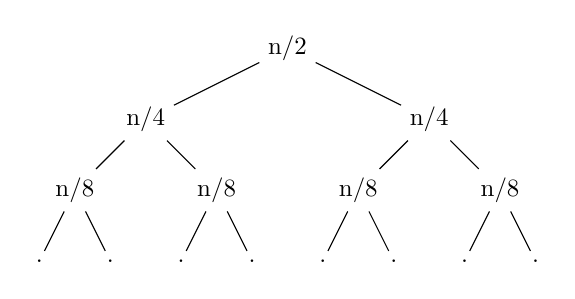
\begin{tikzpicture}[scale=.9, transform shape]

\tikzstyle{every node} = [rectangle, fill=gray!0]

\node (s) at (1,0) {.};
\node (t) at (2,0) {.};
\node (u) at (3,0) {.};
\node (v) at (4,0) {.};
\node (w) at (5,0) {.};
\node (x) at (6,0) {.};
\node (y) at (7,0) {.};
\node (z) at (8,0) {.};

\node (a) at (1.5,1) {n/8};
\node (b) at (3.5,1) {n/8};
\node (c) at (5.5,1) {n/8};
\node (d) at (7.5,1) {n/8};

\node (e) at (2.5,2) {n/4};
\node (f) at (6.5,2) {n/4};

\node (g) at (4.5,3) {n/2};

\draw[-] (s) -- (a);
\draw[-] (t) -- (a);
\draw[-] (u) -- (b);
\draw[-] (v) -- (b);
\draw[-] (w) -- (c);
\draw[-] (x) -- (c);
\draw[-] (y) -- (d);
\draw[-] (z) -- (d);

\draw[-] (a) -- (e);
\draw[-] (b) -- (e);
\draw[-] (c) -- (f);
\draw[-] (d) -- (f);

\draw[-] (e) -- (g);
\draw[-] (f) -- (g);
\end{tikzpicture} 
\caption{Recursion tree for quicksort writes}
\label{fig:rec_tree}
\end{figure}

\textbf{PCM write analysis}: 
Given an array with randomly permuted $N_R$ elements, let us assume the chosen pivot in each phase of recursion is the median of the partition elements. Since the elements are arranged randomly, the probability that the element is in the right partition is $1/2$. In other words, $n/2$ elements are expected to be incorrectly placed.

If Hoare partitioning \cite{cormen} is used, wherein each misplaced element is swapped with another misplaced element. moving these elements to their right partitions will incur $n/2$ writes. In the next level of the recursion tree, there will be $n/4$ writes for both the partitions, again totalling to $n/2$. Thus, $n/2$ writes for swaps will continue until the size of the partition reaches to less than $D$, i.e when the level $l = \lceil log_2 (\frac{N_R L_R}{D}) \rceil$. After this, there would simply be $N_R L_R$ writes for writing each each sorted partition. This recursion tree is shown in Figure \ref{fig:rec_tree}. Totalling this across all levels, we get:
\begin{equation}
\label{eq:sort_conv}
\begin{split}
W_{sort\_conv} = 0.5N_RL_R \lceil log_2(\frac{N_R L_R}{D}) \rceil + N_R L_R\\
  = N_RL_R (0.5 \lceil log_2(\frac{N_R L_R}{D}) \rceil + 1) \\
\end{split}
\end{equation}



\begin{comment}
In the quicksort algorithm on randomly permuted $N_R$ tuples, the average number of swaps is $0.33N_Rln(N_R)$ \cite{swaps}. If each pair of swapped tuples gets evicted from DRAM to PCM after each intermediate swap, there will be two tuple writes (of $L_R$ bytes each) in PCM per pair of swapped tuples. Hence, the total number of writes is given by:  
\end{comment}
\subsection{Multi-pivot quicksort}
\label{subsec:sort_mpivot}
It is clear from the discussion on conventional sorting that, in terms of writes, the faster we converge to partition sizes within DRAM size, the better. A limitation of the conventional quicksort algorithm is that partitioning using a single pivot leads to just two partitions. Thus, with each recursive step in quicksort, the partition size is at best halved (assuming selecting the median as the pivot each time). The intuition behind the multi-pivot quicksort algorithm is to get past this limitation of single-pivot quicksort by using multiple pivots instead, so that the individual partitions quickly converge to a size lesser than the DRAM size.

However, in the multi-pivot case, we do not have any prior information about the endpoints of the partitions to facilitate direct movement of elements to their respective partitions during partitioning, as is done in single pivot quicksort. We address this limitation by adding a separate \textit{read phase} that makes an initial read pass over the input elements counting the number of elements between each consecutive pair of pivots. Note that these counters, by virtue of being continuously updated during the read pass, are likely to be updated within DRAM itself, not incurring PCM writes. After this pass, we are equipped with the endpoint information necessary for the subsequent phases of the algorithm.

We now present an exposition of the various phases of the multi-pivot quicksort algorithm:

\subsubsection{Read phase} 



In the read phase, we divide the input tuples into $p$ partitions of approximately D size each s.t. $p = \lceil \frac{N_R L_R}{D} \rceil$ by choosing $p-1$ random tuples as pivots. These pivots are then copied to a separate location and sorted. Subsequently, we scan through the tuples array counting the number of elements between each consecutive pair of pivots. This is accomplished by doing a binary search within the sorted list of pivots for each tuple in the array. Algorithm \ref{alg:read_phase} represents the pseudo-code for the read phase.

\begin{algorithm}
%{\fontsize{8pt}{10pt}\selectfont
\caption{Read Phase}
\label{alg:read_phase}
\textbf{c} is a design parameter\\
\begin{algorithmic}[1]
\State p = $\lceil c\times \frac{N_R L_R}{D} \rceil$;
\State randIndex[] = generate $p-1$ random indexes;
\State pivot[] = a[randIndex];
\State size[] = {0..0};   
\Comment{size of sub-arrays}
\For {i=$1$ to $N_R$}
\State partition = getPartition(array[i]) 
\State size[partition]++ 
\EndFor
\Comment {Time complexity=$N_R\times log_2p$ }
\State Calculate the boundary index of sub-arrays using their size.
\State return sub-arrays boundary indexes;
\end{algorithmic}
%}
\end{algorithm}


\subsubsection{Swap phase} 
The swap phase uses the information gathered in the read phase to group tuples of the same partition together. The algorithm for swap phase is shown in Fig \ref{alg:swap_phase}. The algorithm operates in a manner similar to cycle-sort, writing each entry directly to its correct partition in-place. 

The algorithm first picks up a wrongly placed entry $e_1$ in a partition $P_1$ and determines it's correct partition $P_2$ by comparing it with the pivots. It then finds another wrongly placed entry $e_2$ belonging to partition $P_2$ and writes $e_1$ in its place. Now the correct partition $P_3$ of $e_2$ is determined and a misplaced element $e_3$ is identified from $P_3$ as a victim for replacement. The algorithm proceeds in the same manner till the cycle completes with the last incorrectly placed entry belonging to partition $P_1$. The algorithm keeps initiating such cycle of replacements till all the elements are placed in their correct partitions. This is reminiscent of the the cycle-sort algorithm \cite{cycle_sort}.

The pseudo-code for swap phase is shown in Algorithm \ref{alg:swap_phase}. The writes during this phase cannot exceed $N_R L_R$ since in the worst case, \emph{each} tuple would have to be moved to its correct partition.

\begin{algorithm}[h!]
%{\fontsize{8pt}{10pt}\selectfont
\caption{Swap Phase}
\label{alg:swap_phase}
partitionStart[] and partitionEnd[] are obtained from Read Phase
\begin{algorithmic}[1]
\For {i=1 to $N_R$}
	\State partitionCorrect = getPartition(array[i])
     \If {i between partitionStart[partitionCorrect] and partitionEnd[partitionCorrect]}                
     \State partitionStart[partitionCorrect]++
	\State continue;
     \Else
			\State presentVictim = a[partitionStart[partitionCorrect]]             
            \State a[partitionStart[partitionCorrect]] = a[i]
            \State partitionStart[partitionCorrect]++
            \State flag = 1;
            \While {flag} 
                \State partitionStart = partitionStart[partitionCorrect];
                \State partitionEnd = partitionStart[partitionCorrect + 1];
                \State partitionLast = partitionCorrect;
                \For {k=partitionStart to partitionEnd} 
                \State partitionCorrect = getPartition(array[i]);
                    \If {k between partitionStart[partitionCorrect] and  partitionStart[partitionCorrect + 1]}
                        \State continue;
                        
                    \ElsIf {k == firstVictimLoc} 
                        \State flag = 0;
                    \EndIf
                    \State swapTuples(presentVictim, array + (arrayElemSize * k));
                    \State currPartitionPtr[partitionLast] = k;
                    \State break;
             
				\EndFor
			\EndWhile
	\EndIf
\EndFor
\Comment {Time complexity=$N_R\times log_2p$ }
\end{algorithmic}
%}
\end{algorithm}


\subsubsection{Sort phase}
Finally, each of the partitions are sorted separately using conventional quicksort to get the final PCM sorted array. If all the partitions are within the DRAM size, the sort phase for each partition can potentially finish within the DRAM without any intermediate evictions to PCM. 

\begin{algorithm}
%{\fontsize{8pt}{10pt}\selectfont
\caption{Sort Phase}
\label{alg:sort_phase}
\begin{algorithmic}[1]
\For {i=$1$ to $p$}
\If {size[p] < D}
\State quicksort(partition $p$)
\Else 
\State multi-pivot quicksort(partition $p$)
\EndIf 
\EndFor
\end{algorithmic}
%}
\end{algorithm}

A point to note here is that since we are choosing the pivot values randomly, it is likely that some partitions turn out to be larger than DRAM. We account for this possibility by creating extra partitions. This is done by selecting a constant c (a value of 2 was found to work well experimentally) s.t. now $p = \lceil c \times \frac{N_R L_R}{D} \rceil$. Post the read phase, we identify the adjoining underflow partitions and coalesce them if their total size is within the DRAM size, after leaving some space for bookkeeping information. If some large partitions still remain, we recursively apply the multi-pivot quicksort algorithm to sort them. Smaller partitions, on the other hand, are sorted using the conventional quicksort, since the sorting process is expected to finish within DRAM and hence not cause any intermediate evictions. 

Figure \ref{fig:mpsort} represents all the steps in the sorting of a given input array for multi-pivot quicksort. In the read phase, 30 and 15 are chosen as pivots. These pivots divide the input elements into 3 different ranges: $< 15$, $\geq 15$ and $< 30$, $\geq 30$. The count of elements in each of these ranges is then determined by making a pass over the elements. In the swap phase, the elements are moved to within the boundaries of their respective partitions. The sort phase finally sorts each of these partitions separately.


%\newcolumntype{b}{>{\columncolor{white}}c}
\begin{figure}[h]
	\centering
	\subfloat[Read Phase]{	
  	%\includegraphics[width=8cm]{sort_step_1.png}
  	
  	\begin{tabular}{|c|c|c|y|c|y|c|c|c|}
        \hline
        24&3&33&30&21&15&7&32&11\\\hline
    \end{tabular}
    }
	\hspace{0mm}
	\subfloat[Swap Phase]{
  	\begin{tabular}{|x|x|x|y|y|y|z|z|z|}
        \hline
        11&3&7&24&21&15&33&32&30\\\hline
    \end{tabular}
    }
    \hspace{0mm}
	\subfloat[Sort Phase]{
  	\begin{tabular}{|x|x|x|y|y|y|z|z|z|}
        \hline
        3&7&11&15&21&24&30&32&33\\\hline
    \end{tabular}
    }
	\caption{Multi-Pivot Sort}
	\label{fig:mpsort}
	
\end{figure}
\textbf{PCM write analysis}: Though the partition boundary counters are continuously updated during the Read phase, they are expected to incur very few PCM writes. This is because since all those updates are in quick succession, the counters are unlikely to be evicted from DRAM  \emph{during} the update process. Similarly, negligible writes would be incurred during extracting and sorting the pivots. During the Swap phase, there will be $N_R L_R$ writes since each tuple is written only once while placing it within its partition boundaries. If each partition is within the DRAM size, the Sort phase (for each partition) will finish within DRAM and there will be another $N_R L_R$ upon eventual eviction of sorted partitions to PCM.  Thus, the total writes in this algorithm is be given by 
\begin{equation}\label{eq:mpivot}
  W_{mpivot} = 2N_RL_R
\end{equation}

\subsection{Multi-pivot sort without explicit partitioining}
The multi-pivot algorithm discussed in the previous section incurred $N_R L_R$ writes during the swap phase due to materialization of partitions in-place. If the available PCM size is sufficient to accommodate another copy of the array to be sorted, we can avoid partitioning writes by trading the swap phase for multiple \textit{sort} passes, each pass carrying out the sorting one of the partitions in the array using the additional space available. This space eventually feeds the sorted tuples as input to the parent operator in the query plan tree. 

In each pass, we go over the entire array, copying the elements belonging to one partition to the space and subsequently sort them there, before moving to the next partition. The process of copying would seem to incur writes of itself and would thus apparently be self-defeating. However, in this case, we leverage the DRAM replacement policy by choosing an appropriate partition size which would prevent dirty (written) words from getting evicted. For N-Chance replacement policy, such a partition size would be $\frac{(N-1)}{K}\times D$. This would ensure that the extracted partition elements do not get evicted before sorting finishes for the partition. In this manner, each partition is processed sequentially by making multiple passes over the entire input array.

\textbf{PCM write analysis}: In this scheme, since there are no extraction writes, the writes incurred are just due to the eviction of the sorted partitions from DRAM. Thus the total writes are given by 
\begin{equation}\label{eq:mpivot_wep}
  W_{mpivot_wep} = N_RL_R
\end{equation}
\section{Hash Join}
\label{hj}

Hash join is another workhorse operator in database systems used most frequently among all join operators. A hash table is built on the smaller relation and larger relation tuples are used to probe for matching value(s) in the join column(s)    .

During the progress of hash join, writes are incurred during building of the hash table, besides during writing of the join results. We discuss the conventional hash table construction followed by our optimisations in the following subsections. We assume $size_{entry}$ as the hash table entry size for each smaller relation tuple. $J$ join output tuples of size $size_{j}$ each would incur $J \times size_{j}$ writes which is common to all the algorithms.

\subsection{Conventional hash table}
Each entry in a hash table consists of a pointer to the corresponding inner table tuple and the hash value for the join columns. To save memory space wastage, typically a separate entry sized space is allocated for each insertion in a bucket and connected to existing entries using an additional pointer. Such an approach incurs an additional pointer write each time a new entry is inserted.

\textbf{PCM write analysis}: Each new entry connects to the previous entry in the bucket by means of a pointer. This would incur $P$ writes apart from $size_{entry}$ writes for each entry. Thus the total writes for conventional hash table is given by
\begin{equation}\label{eq:ht_conv}
  W_{ht\_conv} = N_R \times (size_{entry} + P) + J \times size_{j}
\end{equation}

\subsection{Bitmapped page based allocation}
Allocation of space to buckets is done in units of \textit{pages}. A page contains a set of contiguous entries and is connected to another page by means of a pointer. A bitmap is used to indicate whether each entry in the page is vacant or occupied. Each time a bucket runs out of space, we allocate a new page to the bucket. Though such an approach  may lead to space wastage when some of the pages are not fully occupied, we save on valuable pointer writes which are incurred when the space is allocated on a per-entry basis.

\textbf{PCM write analysis}: Assuming there are $E_{page}$ entries per page, there would now be one pointer per $E_{page}$ entries. In such a case, the writes would be 
$$W_{ht\_bitmapped} = N_R \times (size_{entry} + \frac{P}{E_{page}}) + J \times size_{j}$$\\
Since in practice $\dfrac{P}{E_{page}}$ is small, 
\begin{equation}\label{eq:ht_bmp}
 W_{ht\_bitmapped} \approx N_R \times size_{entry} + J \times size_{j} 
\end{equation} 


\subsection{Reducing hash value length}
We can reduce the writes incurred due to storing of the hash value in the hash table by restricting its length to just a single byte. If the hash function distributes the values in each bucket in a perfectly uniform manner, it would be able to distinguish between 256 join column values in a bucket. This would be sufficient if the number of distinct values mapping in each bucket is not larger than this value. Otherwise, we would have to incur the penalty (in terms of latency) of reading the actual join column(s) value(s) from PCM due to the possiblity of false positives.

\textbf{PCM write analysis}: Let us assume the original hash value was 4 bytes long. Using a single byte hash value instead, combined with a bitmapped page based hash table would lead to total writes of $W_{ht\_pcm}$ given by
\begin{equation}\label{eq:ht_pcm}
W_{ht\_pcm} = N_R \times (size_{entry} - 3)+ J \times size_{j}
\end{equation}
	
%A third approach takes the middle ground between cycles and writes. If we associate with each tuple pointer a 1 byte hash value, it will prevent fetching each inner relation tuple's join column value for each probe of outer relation. Assuming inner relation tuples are uniformly distributed and the hash function maintains this uniformity in hash values also, the chances of collision of hash values would be  $numtuples in a bucket/2^8 = numTuples/256 $. Then the number of PCM accesses required would be $numTuplesinBucket/256$. 

\section{Group-By}%
\label{gby}

Well known techniques for group-by include \textit{sorting} and \textit{hashing}. The technique used depends both on the constraints mentioned in the operator expression itself as well as on the operator following later in the plan tree.


Sorting is used for group-by when an operator such as \textit{order by} appears later in the plan tree. Another use case for sorting based group-by is for queries with \textit{distinct} clause within the aggregation expression. A sample case in point is the following SQL query:
\begin{verbatim}
	select o.customer, count(distinct(o.orderID))
	from orders as o 
	group by o.customer
\end{verbatim}


In such a case, we can now no longer simply update the aggregate values in the hash table for group-by since the existence of duplicates needs to be checked in parallel. To get past this limitation, query optimisers usually choose to use sorting for aggregation. Since the group of tuples forming each aggregate now reside contiguously in the sorted list, duplicates can be identified easily and eliminated, while performing the aggregation.

In the rest of the cases, it is hashing which is the method of choice by virtue of having lesser time complexity in comparison to sorting; the hash table construction being close to that of hash join but with a few differences.

In the following subsections, we start with the conventional group-by operator based on sorting and hashing and later present techniques to achieve a reduction in the writes. We assume that there are $G$ groups in the relation with $size_g$ as the size of each output aggregate tuple. For hash based group-by, $size_{agg\_field}$ represents the size of the aggregate field during grouping and $size_{entry}$ is the hash table entry size for each tuple. The additional writes $G \ times size_g$ of writing out the aggregate tuples themselves after finishing with sorting/hashing  is common to all the techniques presented.

\subsection{Conventional group-by}


A hash table entry for group-by, as compared to hash table entry in hash join, is accompanied by an additional field of aggregate value. For each new tuple in the input array, a bucket index is obtained after hashing the value(s) of the column(s) featuring in the group-by expression. Subsequently, a search is made in the bucket indicated by the index. If a tuple matching in the group-by column(s) value is found, the aggregate field value is updated; else, a new entry is created in the bucket. Thus, unlike hash join where each smaller relation tuple has an entry of its own, the grouped tuples share a common entry with an aggregate field that usually keeps getting updated over the course of the algorithm.

\textbf{PCM write analysis}: For sort based grouping, the writes would be akin to those incurred for sorting. If there are $0.33nln(n)$ \cite{swaps} swaps and each such intermediate swapped pair gets evicted, there will be $2 \times 0.33nln(n)$ writes. Thus, the total writes in our case would be:
\begin{equation}
\label{eq:gby_conv_sort}
W_{gb\_conv\_sort} = 0.66 N_R L_R ln(N_R) + G \times size_g
\end{equation}	

In hash table based group-by, the number of separate entries in the hash table would be $G$, incurring $G \times size_{entry}$ writes. The writes due to updation on the other hand would be $N_R \times size_{agg\_field}$ assuming each intermediate update gets evicted. This would give a total writes of:

\begin{equation}
\label{eq:gby_conv_ht}
\begin{split}
W_{gb\_conv\_ht} = G \times (size_{entry} + P) + \\
N_R \times size_{agg\_field} + G \times size_g
\end{split}
\end{equation}

\subsection{Pointer based multi-pivot quicksort grouping}
\label{subsec:gb_ptr_mpivot} 
Sorting based group-by, as against the sorting operator itself, differs in a key aspect that the sorted tuples themselves are not required to be written out. Instead, it is the aggregated tuples that are finally passed on to the next operator in the plan tree. Hence, in the modified multi-pivot quicksort of Section~\ref{subsec:sort_mpivot}, we use pointers in both the \textit{Swap} and the \textit{Sort} phases and later use those pointers to perform aggregation on the sorted tuples. Thus pointer based multi-pivot quicksort incurs lesser writes than multi-pass multi-pivot quicksort, since the full tuples writes in the latter are replaced by pointer writes in this algorithm.

\textbf{PCM write analysis}: The full tuple writes of $2 N_R L_R$ which were incurred in the original multi-pivot quicksort scheme will now be replaced by by $2N_R \times P$ since pointers are used during both partitioning and sorting phases. Thus, the total writes for this algorithm would be given by:

\begin{equation}
\label{eq:gby_ptr_mpivot}
W_{gb\_ptr\_mpivot} = 2N_R \times P + G \times size_g
\end{equation}

\subsection{Pointer based hashed grouping}

For group-by with \textit{distinct} clause scenarios, we could use the same sorting algorithm as in Section \ref{subsec:gb_ptr_mpivot}. However, in this case, the entire array need not be sorted, which means dividing the array on the basis of pivots can be dropped. In the modified algorithm for group-by, we instead use hashing as the means to divide the input tuples into DRAM sized partitions. These partitions are then sorted by means of pointers, just as in the pointer based multi-pivot algorithm. Though this methodology doesn't reduce the writes from the original pivot based partitioning, it helps bring down the time complexity of moving the tuples to the right partitions. This is because now, we need not perform a binary search within the sorted list of pivots to find out in which range the tuple's join column value belongs. Instead, a direct hash of the join column value can determine the correct partition for the tuple. The modified partitioning pseudo-code is shown in Algorithm \ref{alg:hash_based_pcm_partition}.

\begin{algorithm}[h!]
\caption{Hashing based PCM aware partitioning}
\label{alg:hash_based_pcm_partition}
\textbf{c} is a constant having value between 2 and 3\\
\begin{algorithmic}[1]
\State $ p = c\times \frac{N_R L_R}{D}$;
\State $ size[] = {0..0}$;   
\Comment{size of sub-arrays}\\
\textbf{Read Phase}
\For {$i$=$1$ to $N_R$}
\State Increment the size of sub-array corresponding to $a[i]$; 
\EndFor
\Comment {Time complexity=$N_R$ }
\State Calculate the boundary index of sub-arrays using their size.\\
\textbf{Swap Phase}
\State Swap the pointers to the misplaced elements in sub-arrays in a cycle so that each element is in its correct sub-array;
\Comment {Time complexity=$N_R$ }
\State return sub-arrays boundary indexes;
\end{algorithmic}
\end{algorithm} 

As we can see, hash based partitioning brings down the time complexity of both the read phase and the swap phase to $N_R$ from $N_R \times log_2p$ while retaining the write efficiency of pointer based multi-pivot quicksort grouping. 


\textbf{PCM write analysis}: The expected writes for this algorithm are the same as those of the previous algorithm, i.e. 
\begin{equation}
\label{eq:gby_ptr_hash}
W_{gb\_ptr\_hash} = 2N_R \times P + G \times size_g
\end{equation}

\subsection{Hash table based group-by}
The hash table for group-by is identical to the hash table for hash join apart from an additional aggregate field. Thus, we can apply the same optimizations as we do in hash join in order to reduce the writes during hash table construction. Consequently, the total writes incurred for the optimized hash table case would be given by

\begin{equation}
\begin{split}
W_{gb\_opt\_ht} = G \times (size_{entry} - 3) + \\
N_R \times size_{agg\_field} + G \times size_g
\end{split}
\end{equation}


%\subsection*{Unitary increment based Group-by}
%There can be cases where the Hash Table size is much larger than the DRAM and the group-by aggregate field involves a counter that undergoes unit increments. A sample case in point is the \textit{Count} aggregate function. A simple binary counter can lead to an arbitrary number of writes during intermediate evictions. For e.g., consider a counter having a decimal value of $2$ represented by a 3-bit binary value of $010$. An increment would change it to $011$ incurring a 1 bit write. A subsequent increment however would change it to $100$ leading to 3 bit writes. For such scenarios, we propose counters based on \textit{Gray Codes} \cite{gray_code}. The Gray Code representation between two contiguous count value differs by a single bit. For the previous example, the next gray code value after $011$ will be $111$. Thus, in the case where there is a high probability of each successive count value getting evicted, the writes per eviction would be close to a few bits.

\section{Simulation Testbed}
This section details our experimental settings in terms of the hardware settings, the benchmark queries used as well as the performance metrics on which we evaluated the algorithms.

\label{sec:exp}
\subsection{Architectural Platform}
Since PCM memory is as yet not commercially available, we
have taken recourse to a simulated hardware environment to
evaluate the impact of the PCM-conscious operators.  For this
purpose, we chose Multi2sim~\cite{multi2sim}, an open source
application-only\footnote{Simulates only the application layer without
the OS stack.} simulator that can model a multithreaded, multicore,
superscalar x86 CPU and an AMD Evergreen GPU. It has support for both
functional simulation and cycle-accurate detailed architecture simulation.

Since Multi2sim does not have native support for PCM, we made a major extension to its existing memory module to model PCM memory. A separate architecture
controlled DRAM buffer was included as an additional level in the memory
hierarchy, specifically between the L2 cache and the PCM. We added additional capabilities in the simulator so that the simulated program could ask the simulator to dump intermediate statistics, to know individual operators performance for instance. 

The DRAM was simulated as a set associative write-back memory with \textit{N-Chance}
as the eviction policy. As mentioned in \cite{nchance}, $N$ was set
to $\frac{n}{2}$, where $n$ is the cache associativity, since this
setting was found to provide good performance on multiple metrics -- writes, energy
and latency.  Finally, the timing simulation was modified to account
for the asymmetric read and write latencies of PCM.


\begin{comment}
Since our experiments consider J
In our experiments, we have used $n$ to be 8, therefore making $N$ to be 4.
\end{comment}

Like most other architectural simulators, Multi2sim does not
explicitly track the data residing at the different levels of the
memory hierarchy. It instead maintains only a single buffer that
indicates the latest data, as visible to the simulated program, for
each memory location. We therefore had to add separate data tracking
functionality for the DRAM and PCM resident data. Since we follow
a \textit{read-before-write} policy for DRAM eviction, this addition
enabled us to read the original PCM resident data block and compare
it with the evicted DRAM block, thereby restricting the writes to only
where the data bits differed. In the experiments, we measure writes at
both \textit{bit} and \textit{word} granularities.

Apart from the raw number of writes, a critical related metric for PCM
algorithms is their wear distribution. We therefore instrumented the
Multi2sim code to track block level wear distribution information. To
achieve this, separate counters were created that tracked word (4B)
writes to each location during the query processing activity.

The specific configurations used in the memory hierarchy (L1 Data,
L1 Instruction, L2, DRAM Buffer, PCM) evaluated in our experiments are
enumerated in Table~\ref{table:setup}.  These values are scaled down
versions, wrt number of lines, of the hardware simulation parameters
used in \cite{wear} -- the reason for the scaling down is to ensure
that the simulator running times are not impractically long. However,
we have been careful to ensure that the \emph{ratios} between the sizes
of adjacent levels in the hierarchy are maintained as per the original
configurations in \cite{wear}.

Finally, despite the Multi2sim simulator having support for multiple
threads/processes, we restricted our experiments to a single process with
a single thread of execution. This choice ensured that the entire private
DRAM was available to the executing query. The effect of reduced DRAM
availability due to multiple programs running in parallel was \emph{inferred}
by conducting additional experiments with reduced DRAM sizes, and 
these results are also presented here.

\begin{center}
\begin{table}[htbp]
\begin{small}
\caption{Experimental Setup}
\label{table:setup}
\begin{tabular}{p{2.5cm}p{5.2cm}}
\toprule
Simulator & Multi2sim-4.2 with added support for PCM\\ \hline

L1D cache (private) & 32KB, 64B line, 4-way set-associative, 4 cycle latency, write-back, LRU replacement policy\\ \hline
L1I cache (private) & 32KB, 64B line, 4-way set-associative, 4 cycle latency, write-back, LRU replacement policy\\ \hline   
L2 cache (private) & 256KB, 64B line, 4-way set-associative, 11 cycle latency, write-back, LRU replacement policy\\ \hline

DRAM buffer (private) & 4MB, 256B line, 8-way set-associative, 200 cycle latency, write-back, N-Chance replacement policy (N = 4)\\ \hline

Main Memory & 2 GB PCM, 4KB page, 1024 cycle read latency (per 256B line), 64 cycle write latency (per 4B modified word)\\
\bottomrule
\end{tabular}
\end{small}
\end{table}
\end{center}

\subsection{Database and Queries}
%We used TPC-H (version 2.16.0) 1GB PCM-resident database for our experiments.
For the data, we used the default 1GB database generated by the TPC-H
benchmark.  This size is certainly small compared to the database sizes
typically encountered in modern applications -- however, we again chose
this reduced value to ensure viable simulation running times.

\begin{comment}
Notwithstanding, to ensure that our results were not skewed 
as an outcome,  we used scaled down versions of the hardware simulation parameters
from \cite{wear}, taking care to preserve the size ratios between adjacent
memory devices.
\end{comment}

For simulating our suite of database operators (\textit{sort},
\textit{hash join} and \textit{group by}), we created a separate
library consisting of the native PostgreSQL implementation of these
operators. To this library, we added the PCM-conscious versions described in
the previous sections.


While we experimented with several of the TPC-H queries, results for
three queries: Query 13 (Q13), Query 16 (Q16) and Query 19 (Q19), that
cover a diverse spectrum of the experimental space, are presented here.
For each of the queries, we first identified the query execution plan
recommended by the PostgreSQL query optimizer with the native operators,
and then forcibly used the same execution plan for their PCM-conscious
replacements as well. This was done in order to maintain fairness in the comparison of the PCM-oblivious and PCM-conscious algorithms, though it is possible that a better plan is available. The SQL queries are shown in Figure~\ref{fig:queries}. The specific plans used for these three queries
are shown in Figure~\ref{fig:plan_trees}.

   \lstset{width=\textwidth,
          %frame = single,
          escapechar=@,
          language=SQL,
          basicstyle=\scriptsize
          }

\newsavebox{\firstlisting}
\begin{lrbox}{\firstlisting}% Store first listing
\begin{lstlisting}
select c_count, count(*) as custdist
from ( select c_custkey, count(o_orderkey)
       from customer left outer join orders on 
       c_custkey = o_custkey and 
       o_comment not like '%pending%accounts%'
       group by c_custkey
      ) as c_orders (c_custkey, c_count)
group by c_count
order by custdist desc, c_count desc;
\end{lstlisting}
\end{lrbox}

\newsavebox{\secondlisting}
\begin{lrbox}{\secondlisting}% Store first listing
\begin{lstlisting}
select p_brand, p_type, p_size,
        count(distinct ps_suppkey) as supplier_cnt
from partsupp, part
where p_partkey = ps_partkey
        and p_brand <> 'Brand#35'
        and p_type not like 'ECONOMY BURNISHED%'
        and p_size in (14, 7, 21, 24, 35, 33, 2, 20)
        and ps_suppkey not in ( select s_suppkey
            from supplier
            where s_comment like '%Customer%Complaints%')
group by p_brand, p_type, p_size
order by supplier_cnt desc, p_brand, p_type, p_size;

\end{lstlisting}
\end{lrbox}

\newsavebox{\thirdlisting}
\begin{lrbox}{\thirdlisting}% Store first listing
\begin{lstlisting}
select sum(l_extendedprice* (1 - l_discount)) as revenue
from lineitem, part
where
 ( p_partkey = l_partkey and p_brand = 'Brand#23'
    and p_container in ('SM CASE', 'SM BOX', 'SM PACK', 'SM PKG')
    and l_quantity >= 5 and l_quantity <= 5 + 10
    and p_size between 1 and 5 and l_shipmode in ('AIR', 'AIR REG')
    and l_shipinstruct = 'DELIVER IN PERSON' )
or 
(  p_partkey = l_partkey and p_brand = 'Brand#15'
   and p_container in ('MED BAG', 'MED BOX', 'MED PKG', 'MED PACK')
   and l_quantity >= 14 and l_quantity <= 14 + 10
   and p_size between 1 and 10 and l_shipmode in ('AIR', 'AIR REG')
   and l_shipinstruct = 'DELIVER IN PERSON')
or 
( p_partkey = l_partkey and p_brand = 'Brand#44'
   and p_container in ('LG CASE', 'LG BOX', 'LG PACK', 'LG PKG')
   and l_quantity >= 28 and l_quantity <= 28 + 10
   and p_size between 1 and 15 and l_shipmode in ('AIR', 'AIR REG')
   and l_shipinstruct = 'DELIVER IN PERSON' );
\end{lstlisting}
\end{lrbox}

\begin{figure*}[ht]
\sbox{\measurebox}{
\begin{minipage}[b]{.33\textwidth}
\subfloat[Q13]{\usebox{\firstlisting}}
\hfill%
\subfloat[Q16]{\usebox{\secondlisting}}  
\end{minipage}
}
\usebox{\measurebox}\qquad
\hspace{4em}
\begin{minipage}[b][\ht\measurebox][s]{.33\textwidth}
\subfloat[Q19]{\usebox{\thirdlisting}} 
\end{minipage}
\caption{ Queries}

\label{fig:queries}
\end{figure*}





\subsection{Performance Metrics}
We measured the following performance metrics for each of the queries:
\begin{itemize}
\item number of PCM writes
\item running times (in terms of processor cycles)
\item wear distribution
\end{itemize}
In addition, we measured writes and cycles for each of the
operators invoked during the query execution.

\begin{figure*}[htpb]
\centering
\subfloat[Q13]{
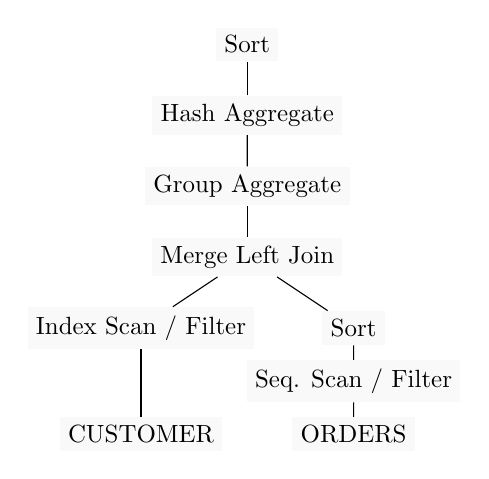
\begin{tikzpicture}[scale=.9, transform shape]

\tikzstyle{every node} = [rectangle, fill=gray!5]

\node (d) at (0,3) {Index Scan / Filter};
\node (c) at (0,1.5) {CUSTOMER};

\node (s) at (3,3) {Sort};
\node (p) at (3,2.25) {Seq. Scan / Filter};
\node (a) at (3,1.5) {ORDERS};

\node (e) at (1.5,4) {Merge Left Join};
\node (f) at (1.5,5)  {Group Aggregate};
\node (g) at (1.5,6)  {Hash Aggregate};
\node (h) at (1.5,7)  {Sort};


\draw[-] (c) -- (d);
\draw[-] (a) -- (p);
\draw[-] (d) -- (e);
\draw[-] (p) -- (s);
\draw[-] (s) -- (e);
\draw[-] (e) -- (f);

\draw[-] (f) -- (g);
\draw[-] (g) -- (h);

\end{tikzpicture}
}
\subfloat[Q16]{
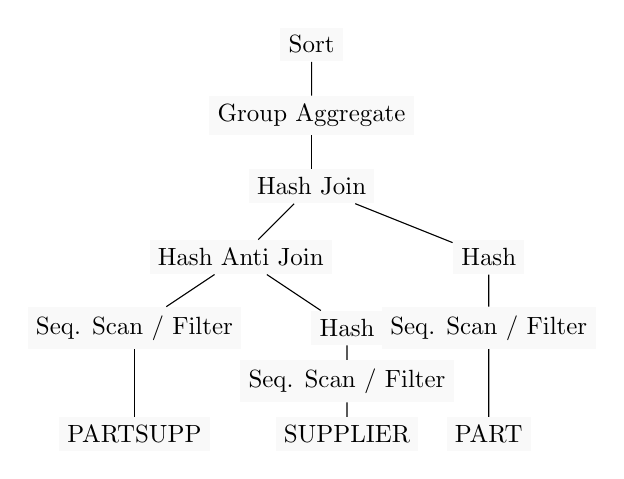
\begin{tikzpicture}[scale=.9, transform shape]

\tikzstyle{every node} = [rectangle, fill=gray!5]

\node (d) at (0,3) {Seq. Scan / Filter};
\node (c) at (0,1.5) {PARTSUPP};

\node (s) at (3,3) {Hash};
\node (p) at (3,2.25) {Seq. Scan / Filter};
\node (a) at (3,1.5) {SUPPLIER};

\node (e) at (1.5,4) {Hash Anti Join};

\node (n) at (5, 4) {Hash};
\node (b) at (5,3) {Seq. Scan / Filter};
\node (x) at (5,1.5) {PART};

\node (f) at (2.5,5)  {Hash Join};
\node (g) at (2.5,6)  {Group Aggregate};
\node (h) at (2.5,7)  {Sort};


\draw[-] (c) -- (d);
\draw[-] (a) -- (p);
\draw[-] (d) -- (e);
\draw[-] (p) -- (s);
\draw[-] (s) -- (e);
\draw[-] (e) -- (f);

\draw[-] (x) -- (b);
\draw[-] (b) -- (n);
\draw[-] (n) -- (f);

\draw[-] (f) -- (g);
\draw[-] (g) -- (h);

\end{tikzpicture}

}
\subfloat[Q19]{


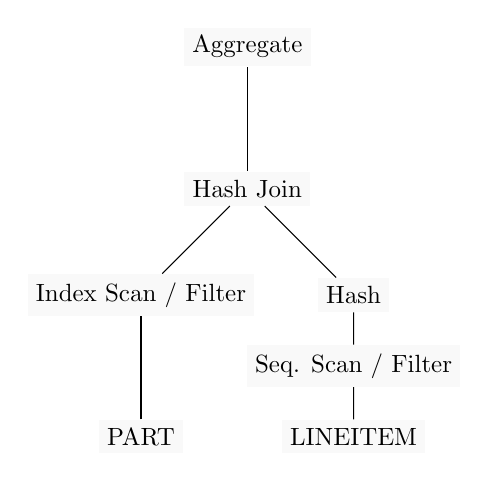
\begin{tikzpicture}[scale=.9, transform shape]

\tikzstyle{every node} = [rectangle, fill=gray!5]

\node (d) at (0,3.5) {Index Scan / Filter};
\node (c) at (0,1.5) {PART};

\node (s) at (3,3.5) {Hash};
\node (p) at (3,2.5) {Seq. Scan / Filter};
\node (a) at (3,1.5) {LINEITEM};

\node (e) at (1.5,5) {Hash Join};
\node (f) at (1.5,7)  {Aggregate};


\draw[-] (c) -- (d);
\draw[-] (a) -- (p);
\draw[-] (d) -- (e);
\draw[-] (p) -- (s);
\draw[-] (s) -- (e);
\draw[-] (e) -- (f);
\end{tikzpicture}
}

\caption{ Query plan trees}

\label{fig:plan_trees}

\end{figure*}
\section{Experimental Results}
\label{sec:results}


We conducted experiments based on the above framework and present
their results in this section. In particular, the PCM Writes and CPU Cycles results of the native
and PCM-conscious executions for Q13, Q16 and Q19 are shown in
Figures~\ref{fig:overall_results_q13}, \ref{fig:overall_results_q16}
and \ref{fig:overall_results_q19}, respectively.
In each of these figures, we provide both the total and the break-ups
on a per operator basis.

\begin{figure}[htbp]
  	\includegraphics[height=29mm]{overall_q13.png}
	\caption{Impact of sort on overall performance - Query 13}
	\label{fig:overall_results_q13}
\end{figure}
Focusing our attention first on Q13 in
Figure~\ref{fig:overall_results_q13}, we find that the bulk of the
overall Writes and Cycles are consumed by the Sort operator. Comparing
the performance of the Native (blue bar) and PCM-conscious (green bar)
implementations, we observe a very significant savings (53\%) on Writes,
and an appreciable decrease (20\%) on Cycles.

\begin{figure}[htbp]
	\centering
	\includegraphics[height=29mm]{overall_q16.png}
	\caption{Impact of group-by on overall performance - Query 16}
	\label{fig:overall_results_q16}
\end{figure}
Turning our attention to Q16 in Figure~\ref{fig:overall_results_q16},
we find that here, it is the group-by operator that primarily influences
the overall Writes performance, whereas the hash-join determines the
Cycles behavior. Again, there are substantial savings in both Writes
(40\%) and  Cycles (30\%) delivered by the PCM-conscious approach.

\begin{figure}[htbp]
	\centering
 	\includegraphics[height=29mm]{overall_q19.png}
	\caption{Impact of hash join on overall performance - Query 19}
	\label{fig:overall_results_q19}
\end{figure}



\begin{comment}
In case of Q13, the running time and writes for the sort operator formed
the bulk of the writes and time taken for the entire query. The group-by
operator comparatively incurred negligible writes and running time. Writes
savings of 53\% and running time savings of 20\% were observed for the
execution of Q13 (shown in sub-figures (a) and (b) resp.) as compared
to native; fuelled mainly by the sort operator.
\end{comment}



\begin{comment}
In case of Q16, both the group-by and hash join operators incurred
significant writes and time. We observed savings of $40\%$ in writes
besides $30\%$ savings in running time as compared to  native algorithms.
\end{comment}

Finally, moving on to Q19 in Figure~\ref{fig:overall_results_q19},
where hash-join is essentially the only operator, we find that the
savings are around $64\%$ with regard to Writes and $32\%$ in Cycles.

We now analyse the savings due to each operator independently, and
show their correspondence to the analysis in Sections~\ref{sort}--~\ref{gby} . 
 
\subsubsection{Sort}

\begin{comment}
The quicksort code from the GNU library was used for the conventional
version of sorting. On the other hand, the PCM-conscious version was
designed to employ a multi-pivot sort when the available DRAM was less
than the size of the data to be sorted; else, it reverted to the
native quicksort algorithm.
For Q13,  where the size of the ORDERS table is 216M, the write ratio
of native single-pivot quicksort to multi-pivot sort is estimated
by the bounds of Section~\ref{sort} to be within
$\displaystyle \frac{2}{2+ln\frac{N_R L_R}{|DRAM|} } \approx
\frac{2}{2+ln\frac {216M}{4M}  } \approx \frac{1}{3}$. These savings
are close to the $XX\%$ depicted by the ratio.
\end{comment}

\begin{comment}
the sort operator was the most heavily used and incurred
the majority of the writes and time. We observed a savings of about
70\% in writes and 20\% in running time. The size of orders table was
216M. 
\end{comment}
For Q13, we observed savings of $53\%$ in writes and $20\%$ in cycles. 

In the case of Q16, the data at the sorting stage was found to be
much lesser than the DRAM size. Hence, both the native and PCM-conscious
executions used the native sort routine, and as a result, the cycles
and writes for both implementations match exactly.

\subsubsection{Hash Join}
Each entry in the hash table consisted of a pointer to the inner tuple
and a hash value field. New memory allocation to each bucket was done in
units of pages, with each page comprised of 64 entries. A search for the
matching join column(s) began with the first tuple in the corresponding
bucket and went on till the last tuple in that bucket, simultaneously
writing out join tuples for successful matches.

For Q16, we observed a $34\%$ improvement in Writes and $12\%$ in Cycles
due to the PCM-conscious hash join, as shown in Figure~\ref{fig:overall_results_q16}. 

These improvements were even higher
with Q19  -- 65\% Writes and 32\% Cycles in Figure~\ref{fig:overall_results_q19} -- the source of the enhancement
was the 3 bytes of writes saved due to single-byte hash values,
in addition to the page-based aggregation of hash table entries.


\subsubsection{Group By}

In Q16, the aggregate operator in the group-by has
an associated \textit{distinct} clause.  Thus, our group-by algorithm
utilized hash-based in-place partitioning followed by sorting to carry
out the aggregation. Both the partitioning and sorting were carried out
through pointers, thereby reducing the writes significantly. Consequently,
we obtain savings of $74\%$ in Writes and $20\%$ in Cycles, as shown in
Figure~\ref{fig:overall_results_q16}.

 

When we consider Q13, however, the hash table consisted of very few entries. The lesser number of entries led to the overhead of page metadata itself overshadowing the savings obtained in other aspects. Specifically, improvements of
about 4\% and 1\% were obtained for Writes and Cycles, as shown in
Figure~\ref{fig:overall_results_q13}.

\begin{comment}

The data at this stage of the group-by was about 6 MB. Using the
bounds derived in Equations \ref{eq:gby_conv_sort} and \ref{eq:gby_ptr_hybrid}, the write ratios of the native and
PCM-conscious algorithms would be within $\frac{ \frac{2 \times size_{ptr}}{N_R
L_R} + 1}{2+ln\frac{N_R L_R}{|DRAM|} + 1} = \frac{1}{3+ln\frac {6M}{4M}
} \approx 29\%$, which is in accordance with the empirical savings of 74\%.

\end{comment}

\begin{figure*}[htbp]
\centering

\subfloat[Q13]{
  \includegraphics[width=5.8cm]{wear_q13.png}
}
\subfloat[Q16]{
  \includegraphics[width=5.8cm]{wear_q16.png}
}
\subfloat[Q19]{
  \includegraphics[width=5.8cm]{wear_q19.png}
}
\caption{Queries wear distribution }
\label{fig:wear_dist}
\end{figure*}



\subsection{Lifetime Analysis}
\begin{comment}
In \cite{qureshi}, the ideal lifetime $Y$ of a PCM device with size $S$
GB, $B$ write traffic, and cell endurance $W_{max}$, is given by:

$Y(years) = \frac{W_{max} \times S}{B} \times 2^{-25}$\\
\end{comment}

The above experiments have shown that PCM-conscious operators can
certainly provide substantive improvements in Writes and Cycles. However,
the question still remains as to whether these improvements have been
purchased at the expense of longevity of the memory. That is, are the
writes skewed towards particular memory locations?  To answer this, we
show in Figure~\ref{fig:wear_dist}, the maximum number of writes  across
all memory blocks (as mentioned earlier, we track writes at the block
level (256 bytes) in our modified simulator), for the three TPC-H queries. The x-axis displays the blocks numbers in decreasing order of writes.

We observe here that the maximum writes is considerably more for the
native systems as compared to the PCM-conscious processing. This
conclusively demonstrates that the improvement is with regard to
\emph{both} average case and worst case behavior.


\begin{comment}
Note that it is possible to achieve this lifetime only when the writes
are perfectly levelled across the entire PCM. In practice, however,
there is a degree of skewness in the writes of most algorithms. Due to
this skew, an algorithm might cut short the PCM lifetime considerably
despite doing well on the overall writes, since a particular set of
locations are written to repeatedly. Hence, characterizing the write
skew is fundamental to determining PCM durability.

As mentioned earlier, we track writes at the block level (256B) in our
modified simulator.  In Figure~\ref{fig:wear_dist}, we show the 
write frequencies of the top 100 blocks for the different operators.

As we can see, in the case of hash join, our PCM-conscious algorithms have
almost the same uniform distribution as the native algorithms. though the
initial part of the writes are slightly higher. This is in those cases
when the bitmap used for maintaining the slot occupancy information for
pages in the hash table is evicted intermediately between bit updates,
thereby incurring higher number of writes for that line.

For group-by (using sort), the per block writes due to our algorithms
are consistently lower than the native algorithms by about $39\%$. The
reason for this is that sorting incurs multiple writes for the same
block when all the input tuples cannot fit in DRAM, which the aspect of
partitioning saves in our PCM-conscious algorithms.

\begin{figure}[htbp]
	\psfig{figure=wear_dist.png, width = 9cm}\centering
	\caption{Operators Wear Distribution }
	\label{fig:wear_dist}
\end{figure} 
\end{comment}

\subsection{DRAM size sensitivity analysis}
We now move on to covering the scenario wherein the available DRAM
size at runtime is lesser than that anticipated prior to the query
execution -- for example, due to concurrent query processing. 
To model this scenario, we experiment with DRAM sizes of 512 KB, 1 MB and
2 MB. Note that, for each of these cases, all the algorithms continue to assume 4 MB as the available DRAM size, oblivious to the actual reduction in the availability of DRAM, and hence continue to execute accordingly. The results are shown in Figures~\ref{fig:sort}, \ref{fig:join}
and \ref{fig:gby} for the Sort, Hash Join and Group By operators, respectively.

In Figure~\ref{fig:sort}, we observe that the Sort operator provides average savings
for Q13 of about 47\% in Writes and 20\% in Cycles.

\begin{figure}[h]
	\centering
	\includegraphics[height=29mm]{sort_q13.png}
    \caption{Sort (Q13)}
	\label{fig:sort}
\end{figure}






%\subsubsection{Sort}

\begin{figure}[h]
	\centering
	\subfloat[Q16]{	
  	\includegraphics[height=29mm]{hj_q16.png}
	}
	\hspace{0mm}
	\subfloat[Q19]{
  	\includegraphics[height=29mm]{hj_q19.png}
	}
	\caption{Hash Join}
	\label{fig:join}
\end{figure}
In case of Q16, the hash join operator rendered $17\%$ improvement in
writes and $50\%$ in running time. The hash join in Q19 continued to benefit with savings of about $42\%$ in writes and again $50\%$
in running time.

\begin{figure}[htbp]
\centering
\subfloat[Q13]{
  \includegraphics[height=29mm]{gb_q13.png}
}
\hspace{0mm}

\subfloat[Q16]{
  \includegraphics[height=29mm]{gb_q16.png}
}
\caption{Group By}
\label{fig:gby}
\end{figure}
For the group-by operator in Q16, writes savings of $78\%$ and running time savings of $26\%$
were observed for the group-by operator. The hash table for group-by being much smaller than all DRAM variants for Q13, the
change in the DRAM size didn't reflect much of a change in writes and
running time - yielding the same average of 4\% and 1\% for the two
metrics respectively.


Thus, we can conclude that the savings obtained by our algorithms are
not restricted to the environment where the DRAM is exclusively available
to one process. Instead, our algorithms can handle the unpredictability
in the DRAM availability due to multiple running processes equally well,
thereby being sufficiently robust to volatile system behaviour.

\subsection{Validating Write Estimators}
\label{validation}
\subsubsection{Sort}

The size of the $orders$ table was approximately $214 \times 10^6$. The conventional quicksort algorithm for Q13 incurred writes of $233.6 \times 10^6$ words $= 934.4 \times 10^6 $bytes. Using Equation \ref{eq:sort_conv}, the expected number of writes were: \\
\begin{dmath}
W_{sort\_conv}(bytes) = N_RL_R (0.5 \lceil log_2(\frac{N_R L_R}{D}) \rceil + 1) \\
= 214 \times 10^6 (0.5 \lceil log_2(\frac{214 \times 10^6}{4 * 10^6}) \rceil + 1) \approx 829.3 \times 10^6 
\end{dmath}
\\
The PCM-conscious version used multi-pivot sort algorithm and incurred writes of $110.6 \times 10^6$ words $= 441.8 \times 10^6 $ bytes. Replacing the values for $N_R L_R$ in Equation \ref{eq:mpivot}, we get the writes as $$W_{mpivot}(bytes) \approx 2 \times 214 \times 10^6  = 428 \times 10^6 $$
Thus both the estimates are close to the observed writes.

\subsubsection{Hash Join}
For hash join in Q19, the values of $N_R$, $size_{entry}$, $J$, $size_{j}$ were $2 \times 10^5$, $8$, $120$ and $8$, respectively. 

The observed writes for PCM-oblivious hash join were $0.90 \times 10^6$ words $= 3.6 \times 10^6$ bytes. Putting the parameter values in Equation \ref{eq:ht_conv}, we get estimated writes as: \\
\begin{dmath}
W_{ht\_conv}(bytes) = N_R \times (size_{entry} + P) + J \times size_{j} =  2 \times 10^5 (8+4) + 120 \times 8 \approx 2.4 \times 10^6 
\end{dmath}
\\
 Using Equation \ref{eq:ht_pcm} for the estimated writes in Q19 for our PCM-conscious version of Hash Join and replacing the  parameter values, the writes are given by:  
$$W_{ht\_pcm}(bytes) = 2 \times 10^5 (8-3) + 120 \times 8 \approx 10^6$$ which is close to the obtained writes of $0.32 \times 10^6$ words $= 1.28 \times 10^6$ bytes.

\subsubsection{Group-By}
The values of the parameters $N_R$, $L_R$, $P$, $G$ and $size_g$ for Q16 were $119056$, $48$, $4$, $18341$ and $48$ respectively.
The observed writes for group-by for PCM-oblivious algorithm were $1.36 \times 10^6$ words $= 5.44 \times 10^6$ bytes. Using Equation \ref{eq:gby_conv_sort} and replacing the parameter values, we get:
\\
\begin{dmath}
W_{gb\_conv\_sort}(bytes) = N_RL_R (0.5 \lceil log_2(\frac{N_R L_R}{D}) \rceil + 1) + G \times size_g = 119056 \times 48  (0.5 \lceil log_2(\frac{119056 \times 48}{4 \times 10^6}) \rceil + 1) + 18341 \times 48
\approx 8 \times 10^6
\end{dmath}
\\
Using Equation \ref{eq:gby_ptr_hash} for write estimation in pointer based hashed grouping algorithm gives us:
\\
\begin{dmath}
W_{gb\_ptr\_hash}(bytes) = 2N_R \times P + G \times size_g
= 2 \times 119056\times 4 + 18341 \times 48
= 1.83 \times 10^6 
\end{dmath}
\\
This closely corresponds to the observed writes of $0.36 \times 10^6$ words $= 1.44 \times 10^6$ bytes.

Thus, our estimators predict writes with a reasonable degree of accuracy for both the PCM-oblivious and PCM-conscious algorithms. Thus, they can be incorporated in the query optimizer to help estimate the writes for a given query plan.

\begin{comment}
\begin{table}[!h]
\centering
\caption{Overview of previous work on operators for PCM }
\label{tab:prev_work}
\begin{small}
\begin{tabular}{p{1.5cm}p{2.3cm}p{1.5cm}p{2cm}}
\toprule  
\textbf{Work} & \textbf{Model} &  \textbf{Operators} & \textbf{Write Guarantees}\\ 
\midrule
Chen et al. \cite{chen} & \textit{PCM\_DRAM} & B$^+$-tree, Hash Join & Hash join writes\\ \hline

Vamsikrishna et al. \cite{vamsi} & \textit {DRAM\_EXPLICIT} & Sort & Writes for basic version of PCM-aware sort\\ \hline

Viglas \cite{viglas} & \textit {DRAM\_EXPLICIT} & Sort, Join & Analysis of a subset of the algorithms presented based on some notion of relative read / write cost\\ 
\bottomrule
\end{tabular}
\end{small}
\end{table} 

\begin{table}[!h]                                                                                       
\centering                                                                                              
                                                                                                          
                                                                                                          
\caption{Validation of write estimators}
  \label{tab:tab_writes}                                                                                
  %\centering                                                                                             
  \begin{small}                                                                                           
  \begin{tabular}{p{2.25cm}p{1.4cm}p{1.6cm}p{1.6cm}}
  \toprule                                                                                                
  
  \textbf{Operator} & \textbf{Equation} & \textbf{Parameter Values} & \textbf{Esimated Writes} & \textbf{Observed Writes}\\
  \midrule                                                                                                
  
  \textbf{Sort PCM-Oblivious} & Equation \ref{eq:sort_conv} \\ 
  
  \textbf{Write energy} & 1.2 J/GB & 6 J/GB  & 65 J/GB \\   
  
  \textbf{Idle power} & $\sim$100 mW/GB & $\sim$1 mW/GB  & $\sim$10 W/TB \\ 
  
  \textbf{Endurance} & $\infty$ & $10^6 - 10^8$  & $\infty$ \\                                            
  
  \textbf{Page size} & 64B & 64B  & 512B \\                                                               
  
  \textbf{Page read latency}& 20-50ns & $\sim 50ns$  & $\sim 5ms$ \\  
  
  \textbf{Page write latency} & 20-50$ns$ & $\sim 1 \mu$s  & $\sim5ms$ \\                                 
  
  \textbf{Write bandwidth}  & $\sim$GB/s per die & 50-100 MB/s per die  & $\sim$200 MB/s per drive \\ 
  
  \textbf{Density} & $1\times$ & 2-4$\times$ & N/A \\                                                     
  
  \bottomrule                                                                                             
  \end{tabular}                                                                                           
  \end{small}                                                                                             
  \end{table} 
  \end{comment}
\input{discussion}
\section{Related Work}
\label{relWork}
On the architecture side, buffer management strategies to reduce PCM latency and energy consumption are discussed in \cite{lee}. Wear levelling algorithm are proposed in \cite{wear} that rotate the lines within a circular buffer each time a certain write threshold is reached. A randomized algorithm was introduced to handle the case when the writes are spatially concentrated to enable wear levelling across entire PCM. Techniques to reduce writes by writing back only modified data to PCM upon eviction from LLC/DRAM are presented in \cite{qureshi, write, lee, zhou}. In Flip-N-Write scheme \cite{flipnwrite}, a modified data word or its complement is stored depending on whose Hamming distance to the original word is lesser. As a result, it restricts the maximum bit writes per word to $B/2$, where \textit{B} is the number of bits in a word.

On the database algorithms front, \cite{cost_aware} seeks to build the PCM read-write asymmetry information within the query optimizer itself. This is orthogonal to our work since we try to optimise for writes during the query execution stage. Writes reduction for B$^+$ Tree index and hash join for \modelPcmRam{} model are proposed in \cite{chen}. It recommends keeping the keys unsorted at the leaf nodes of the index. This would incur extra search time in the leaf nodes but save writes. For partitioning during hash join, a pointer based partitioning approach is proposed to avoid full tuple writes. Since we assume database to be PCM-resident, the partitioning step is obviated in our algorithms. 

Sort and join algorithms for system model \modelExplicit{} are presented in \cite{viglas}. Two classes of algorithms have been proposed for both sort and join. The first class of algorithms divides the input into write incurring and write limited parts. The write incurring part finishes in a single pass whereas the write limited part finishes in  multiple iterations. In the second class of algorithms, the materialization of intermediate results is deferred until the read cost (in terms of time) exceeds the write cost. Our work differs from this work since, unlike their model, our model has no explicit control over DRAM. This means that we cannot selectively decide what to keep in DRAM at any point of time. It also implies that we may ultimately end up getting much lesser DRAM space than we had anticipated, due to other programs running in parallel on the system. As shown in Section \ref{sec:exp}, our algorithms have been designed in such a way that even in the worst case availability, we would do better than conventional algorithms in terms of writes. However, if we consider the sorting algorithms proposed there such as the \textit{lazy sort} algorithm, it uses a heap that may keep constantly getting updated in each pass. If the available DRAM happens to be lesser than the heap size, it is likely that the updated entries keep getting evicted causing a large number of writes. Secondly, the join algorithms proposed there involve partitioning the data for the hash table to fit in DRAM. However, since the results are written out simultaneously with the join process, and given the output tuples count for join can be multiplicative (i.e. if $M$ and $N$ is the cardinality of the input relations, there can potentially be $MN$ output tuples), it is likely that, unless the partitions are very small, the hash table gets evicted even after partitioning. 

Sorting algorithms for \modelExplicit{} model are discussed in \cite{vamsi}. They split the given range into buckets such that each bucket can be sorted using DRAM. The bucket boundaries are determined using hybrid histograms having both depth bound and width bound buckets, the bound being decided depending upon which limit is hit \textit{later}. The elements are then shuffled to group same bucket elements together followed by sorting each bucket using DRAM. The sorting methodology used is quicksort or count sort based on whether the bucket is depth bound or width bound respectively. A major drawback with this approach is that there is a large likelihood of an error in the approximation of the histogram, leading to DRAM overflow in some of the buckets. This would lead to additional writes since the buckets then need to be split. Besides, the construction of a histogram itself incurs writes of its own.

\begin{comment}
Table \ref{tab:prev_work} summarises the previous work on PCM-conscious database operators algorithms.
\end{comment}
There has been related research to speed up query execution for \textit{flash} resident databases. The use of a column based layout has been advocated in \cite{graefe} to avoid fetching unnecessary attributes during scan. The same layout is also leveraged for joins by fetching only the columns participating in the join, deferring full tuple materialization to as late as possible in the plan tree. External Merge sort is recommended for data not fitting in DRAM. These techniques, though applicable to a PCM setting, are orthogonal to our work.
\section{Conclusion and Future Work}
\label{conclusion}
Database query execution algorithms on Phase Change Memory calls for a change in perspective from the conventional algorithm design assumption of symmetric reads and writes. We demonstrate that with carefully designed algorithms, we can leverage the favourable performance of PCM \textit{reads} to cut down on not only the \textit{writes} but the running time as well. 

Even within the class of PCM conscious algorithms, there exist myriad algorithm design choices offering varying degrees of writes and running time. Nested loops join, as shown in Section \ref{tradeoff}, would incur the least amount of writes for join when both relations fit in PCM, but might prove to be extremely slow. Similarly, selection sort trades writes for extra read cycles as compared to multi-pivot quicksort. 

We need to come up with metrics that can quantify this trade-off based upon some measure of the lifetime that the PCM memory module is expected to serve and the maximum delay the user is willing to bear. Secondly, these metrics need to be integrated with the query optimizer for it to choose suitable query execution plans for PCM based hardware. We see this as an interesting line of future work.




\bibliographystyle{abbrv}
\bibliography{sigproc}  % sigproc.bib is the name of the Bibliography in this case
% You must have a proper ".bib" file
%  and remember to run:
% latex bibtex latex latex
% to resolve all references
%
% ACM needs 'a single self-contained file'!
%
%APPENDICES are optional
%\balancecolumns

%Appendix A

\end{document}
